

\mode<presentation>
{
  \usetheme{boxes}
  %\useoutertheme{infolines}
  % með efnisyfirliti: Szeged, Frankfurt 
  % án efnisyfirlits: Pittsburgh
  % áhugavert: CambridgeUS, Boadilla
  %\setbeamercovered{transparent} %gegnsætt
  \setbeamercovered{invisible}

\defbeamertemplate*{footline}{infolines theme}
{
  \leavevmode%
  \hbox{%
  \begin{beamercolorbox}[wd=.333333\paperwidth,ht=2.25ex,dp=1ex,center]{author in head/foot}%
  %  \usebeamerfont{author in head/foot}\insertshortauthor~~\beamer@ifempty{\insertshortinstitute}{}{(\insertshortinstitute)}
  \end{beamercolorbox}%
  \begin{beamercolorbox}[wd=.333333\paperwidth,ht=2.25ex,dp=1ex,center]{title in head/foot}%
   % \usebeamerfont{title in head/foot}\insertshorttitle
  \end{beamercolorbox}%
  \begin{beamercolorbox}[wd=.333333\paperwidth,ht=2.25ex,dp=1ex,right]{date in head/foot}%
    %\usebeamerfont{date in head/foot}\insertshortdate{}\hspace*{2em}
    \insertshortlecture.\insertframenumber{} / \insertshortlecture.\inserttotalframenumber\hspace*{2ex} 
  \end{beamercolorbox}}%
  \vskip0pt%
}
\resetcounteronoverlays{rtaskno} %Does not increase counter rtaskno on \pause in beamer


}


\usepackage[english,icelandic]{babel}
\usepackage[utf8]{inputenc}
\usepackage{t1enc}
\usepackage{graphicx}
\usepackage{amsmath}
\usepackage{amssymb}
\usepackage{mathrsfs}
\usepackage{verbatim}
\usepackage{esint}


% RAGNAR SIGURÐSSON
%\usepackage[T1]{fontenc} 
%\usepackage[icelandic]{babel}
\usepackage{latexsym,amssymb,amsmath}
%\usepackage[utf8]{inputenc}
%\usepackage{graphicx}
\usepackage{epstopdf}
\usepackage{verbatim}
\usepackage{array,tabularx,arydshln}
\setbeamertemplate{theorems}[numbered]


\newtheorem{setning}{Setning}
\newtheorem{hjalpar}{Hjálparsetning}
\theoremstyle{definition}
\newtheorem{rithattur}{Ritháttur}
\newtheorem{skilgreining}{Skilgreining}
\newtheorem{daemi}{Dæmi}
\newtheorem{ath}{Athugasemd}

\newcommand\Wider[2][3em]{%
\makebox[\linewidth][c]{%
  \begin{minipage}{\dimexpr\textwidth+#1\relax}
  \raggedright#2
  \end{minipage}%
  }%
}

%counter used for blocks
\newcounter{rtaskno}
\DeclareRobustCommand{\rtask}[1]{%
   \refstepcounter{rtaskno}%
   \thertaskno\label{#1}}

\newcommand{\C}{{\mathbb  C}}
\newcommand{\Z}{{\mathbb Z}}
\newcommand{\R}{{\mathbb  R}}
\newcommand{\N}{{\mathbb  N}}
\newcommand{\Q}{{\mathbb Q}}
\renewcommand{\phi}{\varphi}
\renewcommand{\epsilon}{\varepsilon}
\newcommand{\p}{{\partial}}
\renewcommand{\d}{{\partial}}

% RAGNAR SIGURÐSSON
\newcommand{\nin}{\mbox{$\;\not\in\;$}}
\newcommand{\dive}{\mbox{${\rm\bf div\,}$}}
\newcommand{\curl}{\mbox{${\rm\bf curl\,}$}}
\newcommand{\grad}{\mbox{${\rm\bf grad\,}$}}
\newcommand{\spann}{\mbox{${\rm Span}$}}
\newcommand{\tr}{\mbox{${\rm tr}$}}
\newcommand{\rank}{\mbox{${\rm rank}$}}
\newcommand{\image}{\mbox{${\rm image}$}}
\newcommand{\nullity}{\mbox{${\rm null}$}}
\newcommand{\proj}{\mbox{${\rm proj}$}}
\newcommand{\id}{\mbox{${\rm id}$}}
%\newcommand{\R}{\mbox{${\bf R}$}}
%\newcommand{\C}{\mbox{${\bf C}$}}
\newcommand{\Rn}{\mbox{${\bf R}^n$}}
\newcommand{\Rm}{\mbox{${\bf R}^m$}}
\newcommand{\Rk}{\mbox{${\bf R}^k$}}
\newcommand{\Av}{\mbox{${\bf A}$}}
\newcommand{\av}{\mbox{${\bf a}$}}
\newcommand{\uv}{\mbox{${\bf u}$}}
\newcommand{\vv}{\mbox{${\bf v}$}}
\newcommand{\wv}{\mbox{${\bf w}$}}
\newcommand{\xv}{\mbox{${\bf x}$}}
\newcommand{\zv}{\mbox{${\bf z}$}}
\newcommand{\yv}{\mbox{${\bf y}$}}
\newcommand{\bv}{\mbox{${\bf b}$}}
\newcommand{\cv}{\mbox{${\bf c}$}}
\newcommand{\dv}{\mbox{${\bf d}$}}
\newcommand{\ev}{\mbox{${\bf e}$}}
\newcommand{\fv}{\mbox{${\bf f}$}}
\newcommand{\gv}{\mbox{${\bf g}$}}
\newcommand{\hv}{\mbox{${\bf h}$}}
\newcommand{\iv}{\mbox{${\bf i}$}}
\newcommand{\jv}{\mbox{${\bf j}$}}
\newcommand{\kv}{\mbox{${\bf k}$}}
\newcommand{\pv}{\mbox{${\bf p}$}}
\newcommand{\nv}{\mbox{${\bf n}$}}
\newcommand{\qv}{\mbox{${\bf q}$}}
\newcommand{\rv}{\mbox{${\bf r}$}}
\newcommand{\sv}{\mbox{${\bf s}$}}
\newcommand{\tv}{\mbox{${\bf t}$}}
\newcommand{\ov}{\mbox{${\bf 0}$}}
\newcommand{\Fv}{\mbox{${\bf F}$}}
\newcommand{\Gv}{\mbox{${\bf G}$}}
\newcommand{\Uv}{\mbox{${\bf U}$}}
\newcommand{\Nv}{\mbox{${\bf N}$}}
\newcommand{\Hv}{\mbox{${\bf H}$}}
\newcommand{\Ev}{\mbox{${\bf E}$}}
\newcommand{\Sv}{\mbox{${\bf S}$}}
\newcommand{\Tv}{\mbox{${\bf T}$}}
\newcommand{\Bv}{\mbox{${\bf B}$}}
\newcommand{\Oa}{\mbox{$(0,0)$}}
\newcommand{\Ob}{\mbox{$(0,0,0)$}}
\newcommand{\Onv}{\mbox{$[0,0,\ldots,0]$}}
\newcommand{\an}{\mbox{$(a_1,a_2, \ldots,a_n)$}}
\newcommand{\xn}{\mbox{$(x_1,x_2, \ldots,x_n)$}}
\newcommand{\xnv}{\mbox{$[x_1,x_2, \ldots,x_n]$}}
\newcommand{\vnv}{\mbox{$[v_1,v_2, \ldots,v_n]$}}
\newcommand{\wnv}{\mbox{$[w_1,w_2, \ldots,w_n]$}}
\newcommand{\tvint}{\int\!\!\!\int}
\newcommand{\thrint}{\int\!\!\!\int\!\!\!\int}
\renewcommand{\ast}{{\operatorname{\text{astand}}}}


\usepackage{caption}
%\usepackage{pgfpages}
% \pgfpagesuselayout{2 on 1}[a4paper,border shrink=5mm]

\def\lecturename{Stærðfræðigreining IIB}
\title{\insertlecture}
\author{Sigurður Örn Stefánsson, \href{mailto:sigurdur@hi.is}{sigurdur@hi.is}}
\institute
{
  Verkfræði- og náttúruvísindasvið\\
  Háskóli Íslands
}
\subtitle{Stærðfræðigreining IIB, STÆ205G}
%\subject{\lecturename}

\mode<article>
{
	\usepackage[colorlinks=false,
	pdfauthor={Sigurður Örn Stefánson},
	%pdftitle={Töluleg greining}
	]{hyperref}
  %\usepackage{times}
  %\usepackage{mathptmx}
  \usepackage[left=1.5cm,right=4cm,top=1.5cm,bottom=3cm]{geometry}
}

% Beamer version theme settings

%\useoutertheme[height=0pt,width=2cm,right]{sidebar}
%\usecolortheme{rose,sidebartab}
%\useinnertheme{circles}
%\usefonttheme[only large]{structurebold}


\setbeamercolor{sidebar right}{bg=black!15}
\setbeamercolor{structure}{fg=blue}
\setbeamercolor{author}{parent=structure}

\setbeamerfont{title}{series=\normalfont,size=\LARGE}
\setbeamerfont{title in sidebar}{series=\bfseries}
\setbeamerfont{author in sidebar}{series=\bfseries}
\setbeamerfont*{item}{series=}
\setbeamerfont{frametitle}{size=}
\setbeamerfont{block title}{size=\small}
\setbeamerfont{subtitle}{size=\normalsize,series=\normalfont}


\setbeamertemplate{sidebar right}
{
  {\usebeamerfont{title in sidebar}%
    \vskip1.5em%
    \hskip3pt%
    \usebeamercolor[fg]{title in sidebar}%
    \insertshorttitle[width=2cm-6pt,center,respectlinebreaks]\par%
    \vskip1.25em%
  }%
  {%
    \hskip3pt%
    \usebeamercolor[fg]{author in sidebar}%
    \usebeamerfont{author in sidebar}%
    \insertshortauthor[width=2cm-2pt,center,respectlinebreaks]\par%
    \vskip1.25em%
  }%
  \hbox to2cm{\hss\insertlogo\hss}
  \vskip1.25em%
  \insertverticalnavigation{2cm}%
  \vfill
  \hbox to 2cm{\hfill\usebeamerfont{subsection in
      sidebar}\strut\usebeamercolor[fg]{subsection in
      sidebar}\insertshortlecture.\insertframenumber\hskip5pt}%
  \vskip3pt%
}%

\setbeamertemplate{title page}
{
  \vbox{}
  \vskip1em
  %{\huge Kapitel \insertshortlecture\par}
  {\usebeamercolor[fg]{title}\usebeamerfont{title}\inserttitle\par}%
  \ifx\insertsubtitle\@empty%
  \else%
    \vskip0.25em%
    {\usebeamerfont{subtitle}\usebeamercolor[fg]{subtitle}\insertsubtitle\par}%
  \fi%     
  \vskip1em\par
  %Vorlesung \emph{\lecturename}\ vom 
  \insertdate\par
  \vskip0pt plus1filll
  \leftskip=0pt plus1fill\insertauthor\par
  \insertinstitute\vskip1em
}

%\logo{\includegraphics[width=2cm]{beamerexample-lecture-logo.pdf}}



% Article version layout settings

\mode<article>

\makeatletter
\def\@listI{\leftmargin\leftmargini
  \parsep 0pt
  \topsep 5\p@   \@plus3\p@ \@minus5\p@
  \itemsep0pt}
\let\@listi=\@listI


\setbeamertemplate{frametitle}{\paragraph*{\insertframetitle\
    \ \small\insertframesubtitle}\ \par
}
\setbeamertemplate{frame end}{%
  \marginpar{\scriptsize\hbox to 1cm{\sffamily%
      \hfill\strut\insertshortlecture.\insertframenumber}\hrule height .2pt}}
\setlength{\marginparwidth}{1cm}
\setlength{\marginparsep}{1.5cm}

\def\@maketitle{\makechapter}

\def\makechapter{
  \newpage
  \null
  \vskip 2em%
  {%
    \parindent=0pt
    \raggedright
    \sffamily
    \vskip8pt
    %{\fontsize{36pt}{36pt}\selectfont Kapitel \insertshortlecture \par\vskip2pt}
    {\fontsize{24pt}{28pt}\selectfont \color{blue!50!black} \insertlecture\par\vskip4pt}
    {\Large\selectfont \color{blue!50!black} \insertsubtitle, \@date\par}
    \vskip10pt

    \normalsize\selectfont \@author\par\vskip1.5em
    %\hfill BLABLA
  }
  \par
  \vskip 1.5em%
}

\let\origstartsection=\@startsection
\def\@startsection#1#2#3#4#5#6{%
  \origstartsection{#1}{#2}{#3}{#4}{#5}{#6\normalfont\sffamily\color{blue!50!black}\selectfont}}

\makeatother

\mode
<all>



% Typesetting Listings

\usepackage{listings}
\lstset{language=Java}

\alt<presentation>
{\lstset{%
  basicstyle=\footnotesize\ttfamily,
  commentstyle=\slshape\color{green!50!black},
  keywordstyle=\bfseries\color{blue!50!black},
  identifierstyle=\color{blue},
  stringstyle=\color{orange},
  escapechar=\#,
  emphstyle=\color{red}}
}
{
  \lstset{%
    basicstyle=\ttfamily,
    keywordstyle=\bfseries,
    commentstyle=\itshape,
    escapechar=\#,
    emphstyle=\bfseries\color{red}
  }
}



% Common theorem-like environments

\theoremstyle{definition}
\newtheorem{exercise}[theorem]{\translate{Exercise}}




% New useful definitions:

\newbox\mytempbox
\newdimen\mytempdimen

\newcommand\includegraphicscopyright[3][]{%
  \leavevmode\vbox{\vskip3pt\raggedright\setbox\mytempbox=\hbox{\includegraphics[#1]{#2}}%
    \mytempdimen=\wd\mytempbox\box\mytempbox\par\vskip1pt%
    \fontsize{3}{3.5}\selectfont{\color{black!25}{\vbox{\hsize=\mytempdimen#3}}}\vskip3pt%
}}

\newenvironment{colortabular}[1]{\medskip\rowcolors[]{1}{blue!20}{blue!10}\tabular{#1}\rowcolor{blue!40}}{\endtabular\medskip}

\def\equad{\leavevmode\hbox{}\quad}

\newenvironment{greencolortabular}[1]
{\medskip\rowcolors[]{1}{green!50!black!20}{green!50!black!10}%
  \tabular{#1}\rowcolor{green!50!black!40}}%
{\endtabular\medskip}


\begin{document}

\section{Margföld heildi}


\subsection{Skiptingar} 

\subsubsection{Skilgreining }
Látum $R=[a,b]\times[c,d]$ vera
rétthyrning í planinu.  {\em Skipting} $P$ á rétthyrningnum $R$ felst í
því að taka skiptingar
$$a=x_0<x_1<\cdots<x_m=b\qquad\mbox{og}\qquad
c=y_0<y_1<\cdots<y_n=d$$
 á bilunum $[a,b]$ og $[c,d]$ og nota þær skiptingar til að skipta $R$
 upp í rétthyrninga $[x_i,x_{i+1}]\times [y_j,y_{j+1}]$.  
Ritum $\Delta x_i=x_{i+1}-x_i$ og  $\Delta y_j=y_{j+1}-y_j$.
{\em Norm} skiptingarinnar $P$, táknað með $\|P\|$,  
er skilgreint sem lengd lengstu hornalínu í
   rétthyrningunum $[x_i,x_{i+1}]\times [y_j,y_{j+1}]$.



Skipting $P$ á rétthyrningi $R= [a,b]\times [c,d]$.

\bigskip
 \begin{figure}[h!]
 \centering
            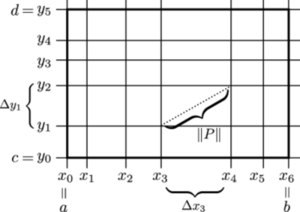
\includegraphics[width=.5\linewidth]{skipting.png}
            \caption*{}
\end{figure}



\subsection{Riemann-summa} 

\subsubsection{Skilgreining }
  
 Látum $f$ vera fall skilgreint á rétthyrningi $R=[a,b]\times[c,d]$ og
 látum $P$ vera skiptingu á $R$.  Veljum úr hverjum rétthyrningi
 $[x_i,x_{i+1}]\times [y_j,y_{j+1}]$ punkt $(x_i^*, y_j^*)$.  
Skilgreinum \emph{Riemann-summuna}
$$\mathcal{R}(f,P)=\sum_{i=1}^m\sum_{j=1}^n f(x_i^*, y_j^*)\Delta x_i\Delta
  y_j.$$

   \begin {figure}[h!]
 \centering
            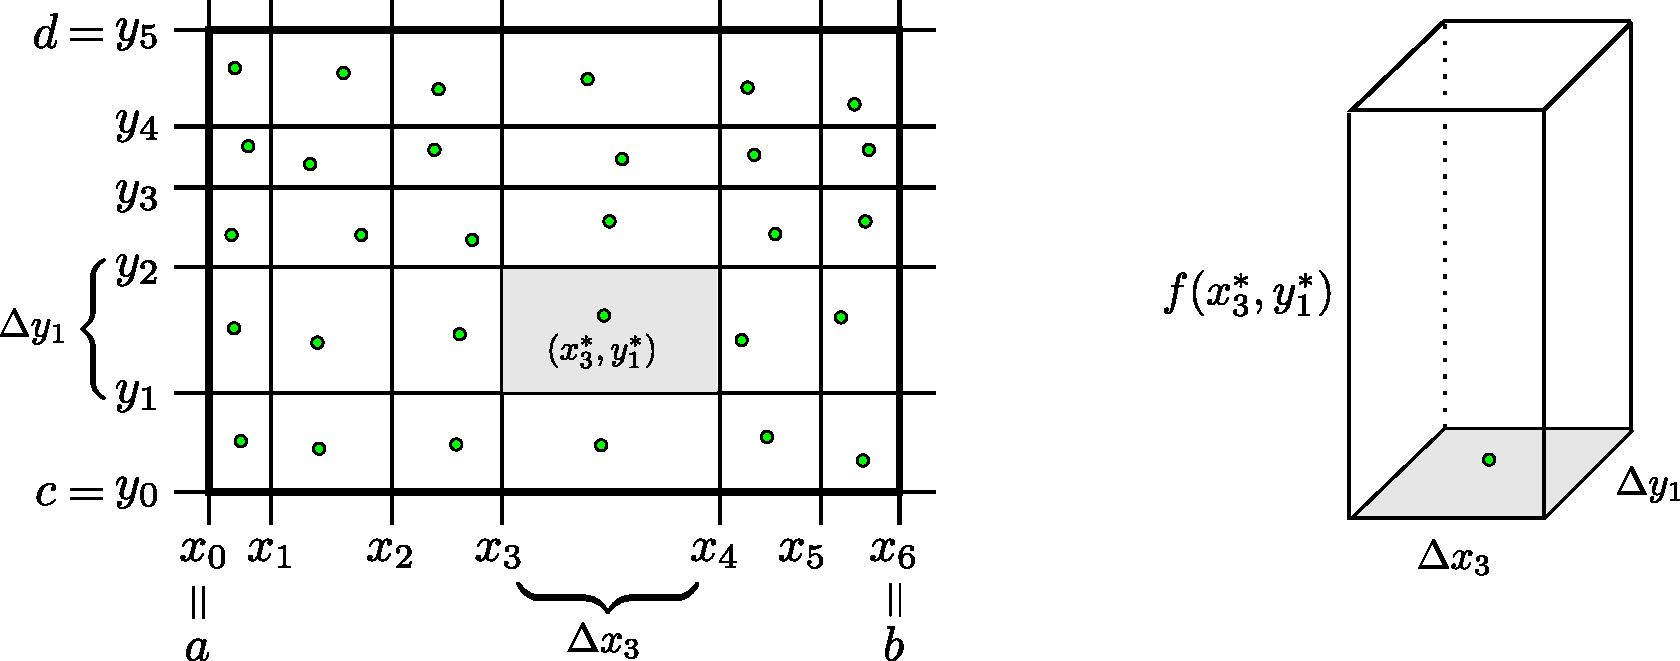
\includegraphics[width=.95\linewidth]{skipting2.pdf}
            \caption*{}
\end {figure}




    \begin {figure}[h!]
 \centering
            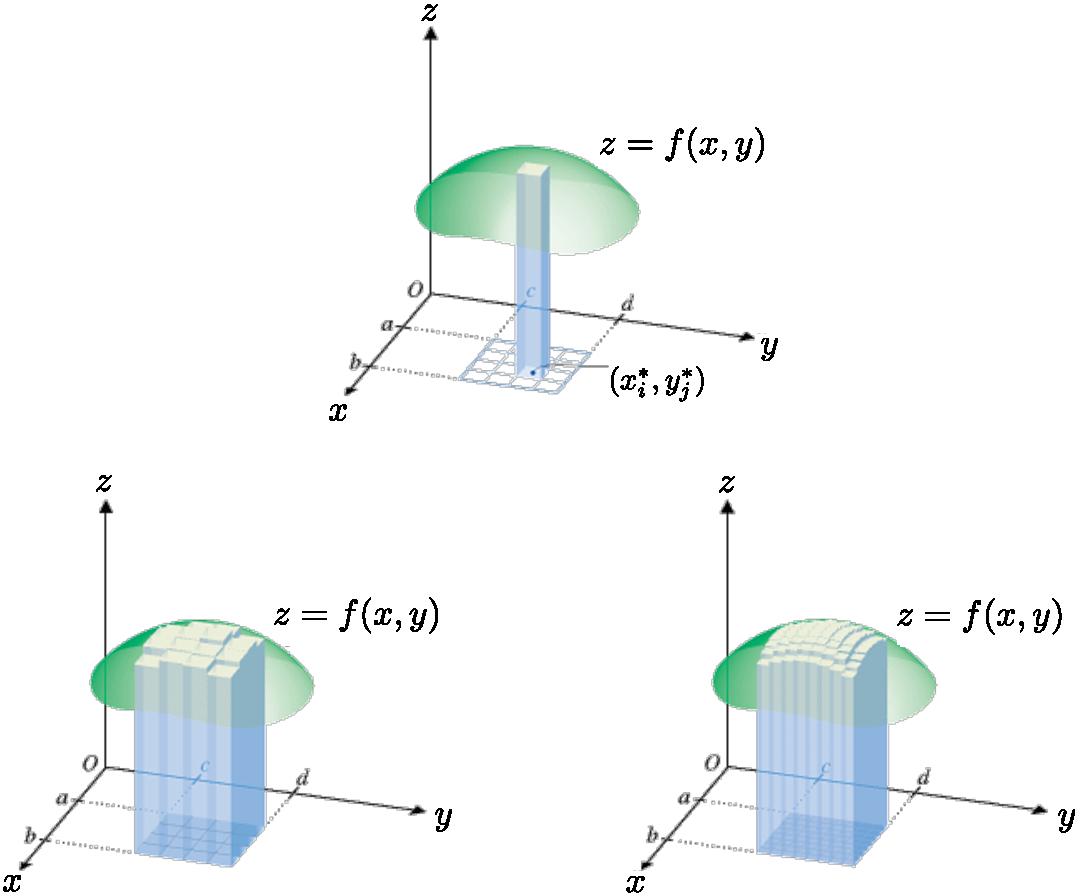
\includegraphics[width=0.9\linewidth]{double.pdf}
            \caption*{}
\end {figure}



\subsection{\nopagebreak Tvöfalt heildi yfir rétthyrning} 

\subsubsection{\nopagebreak Skilgreining }
Sagt er að fall $f$ skilgreint á
rétthyrningi $R=[a,b]\times [c,d]$ sé {\em heildanlegt yfir} $R$ með
heildi $I$ (hér stendur $I$ fyrir tölu) ef fyrir sérhvert
$\epsilon>0$ er til tala $\delta>0$ 
þannig að $|\mathcal{R}(f,P)-I|<\epsilon$ fyrir allar skiptingar $P$ með
$\|P\|<\delta$ óháð vali á punktunum $(x_i^*, y_j^*)$.

Ritum þá 
$$\tvint_R f(x,y)dA=I.$$






\subsection{Tvöfalt heildi yfir takmarkað svæði} 

\subsubsection{Skilgreining }
Látum $D$ vera takmarkað svæði í planinu.
Fall $f$ er sagt heildanlegt yfir $D$ ef til er rétthyrningur $R$ sem
inniheldur $D$ og fallið 
$$\hat{f}(x,y)=\left\{\begin{array}{rcl}
f(x,y)& & \mbox{ef }(x,y)\in D,\\
0& & \mbox{ef }(x,y)\in R\setminus D
\end{array}\right.$$
er heildanlegt yfir $R$.




\subsubsection{Setning }
Látum $f$ vera samfellt fall skilgreint á
lokuðu og takmörkuðu svæði $D$ í planinu $\R^2$.  Gerum ráð fyrir að
jaðar $D$ samanstandi af endanlega mörgum ferlum sem hafa endanlega
lengd.  Þá er fallið $f$ heildanlegt yfir $D$.



\subsubsection{Setning }
Látum $D$ vera svæði í planinu og $f$ takmarkað
fall skilgreint á $D$ og heildanlegt yfir $D$.  Þá gildir:

\begin {enumerate}
 \item $\tvint_D f(x,y)\,dA=0$ ef flatarmál $D$ er 0.
 \item $\tvint_D 1\,dA=$ flatarmál $D$.
 \item Ef $f(x,y)\geq 0$ fyrir alla punkta $(x,y)$ í $D$ þá er 
$\tvint_D f(x,y)\,dA$ jafnt rúmmáli rúmskikans sem liggur milli $D$ og
grafsins $z=f(x,y)$.
\item Ef $f(x,y)\leq 0$ fyrir alla punkta $(x,y)$ í $D$ þá er 
$\tvint_D f(x,y)\,dA$ jafnt mínus rúmmáli rúmskikans sem liggur milli $D$ og
grafsins $z=f(x,y)$.
\end {enumerate}




\subsubsection{Setning }
Ef $D$ er svæði í planinu og $f$ og $g$
heildanleg föll yfir $D$ þá gildir:

\begin {enumerate}
 \item  Ef $L$ og $M$ eru fastar þá er
$$\tvint_D Lf(x,y)+Mg(x,y)\,dA=L\!\tvint_D f(x,y)\,dA+M\!\tvint_D
g(x,y)\,dA.$$
\item  Ef $f(x,y)\leq g(x,y)$ þá er 
$$\tvint_D f(x,y)\,dA\leq \tvint_Dg(x,y)\,dA.$$

\item  Þríhyrningsójafna: 
\scalebox{1}{$\qquad\bigg|\tvint_D f(x,y)\,dA\bigg|\leq \tvint_D |f(x,y)|\,dA.$}

\item  Ritum $D$ sem sammengi af svæðum $D_1,\ldots, D_k$ sem skarast
ekki nema mögulega í jaðarpunktum þá er
$$\tvint_D f(x,y)\,dA=\sum_{i=1}^k\tvint_{D_i}f(x,y)\,dA.$$
\end {enumerate}




\subsubsection{Setning Fubinis }

Látum $f$ vera fall sem er heildanlegt yfir rétthyrning $R=[a,b]\times
[c,d]$. Setjum
\[A(x)=\int_c^d f(x,y)\,dy\qquad\mbox{($x$ hugsað sem fasti þegar heildað)}.\]
Þá gildir að 
\[\tvint_R f(x,y)\,dA=\int_a^b A(x)\,dx=\int_a^b\!\!\int_c^d
f(x,y)\,dy\,dx.\]

Sömuleiðis gildir þegar við setjum 
\[A(y)=\int_a^b f(x,y)\,dx\qquad\mbox{($y$ hugsað sem fasti þegar heildað)} \qquad \text{að}\]
\[\tvint_R f(x,y)\,dA=\int_c^d A(y)\,dy=\int_c^d\!\!\int_a^b
f(x,y)\,dx\,dy.\]



    \begin {figure}[h!]
 \centering
            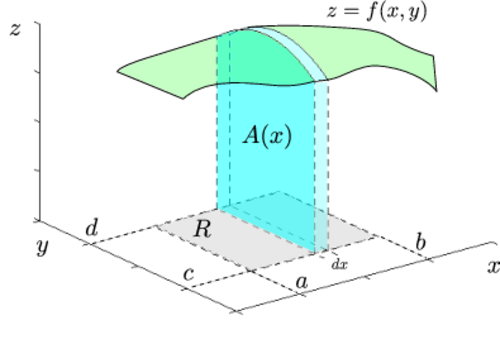
\includegraphics[width=0.6\linewidth]{ax1}
            \caption*{}
\end {figure}



\subsection{$x$-einföld og $y$-einföld svæði} 

\subsubsection{Skilgreining }
Svæði $D$ í planinu er sagt vera $y${\em-einfalt}  ef hægt er að finna tölur $a$ og $b$ og föll $c(x)$ og
$d(x)$ þannig að  
$$D=\{(x,y)\mid a\leq x\leq b, c(x)\leq y\leq d(x)\}.$$
Svæði $D$ í planinu er sagt vera $x${\em-einfalt}  ef hægt er að
finna tölur $c$ og $d$ og föll $a(y)$ og $b(y)$ þannig að  
$$D=\{(x,y)\mid c\leq y\leq d, a(y)\leq x\leq b(y)\}.$$
% SNÝR ÖFUGT MIÐAÐ VIÐ BÓK  Leiðrétta

\begin {figure}[h!]
 \centering
            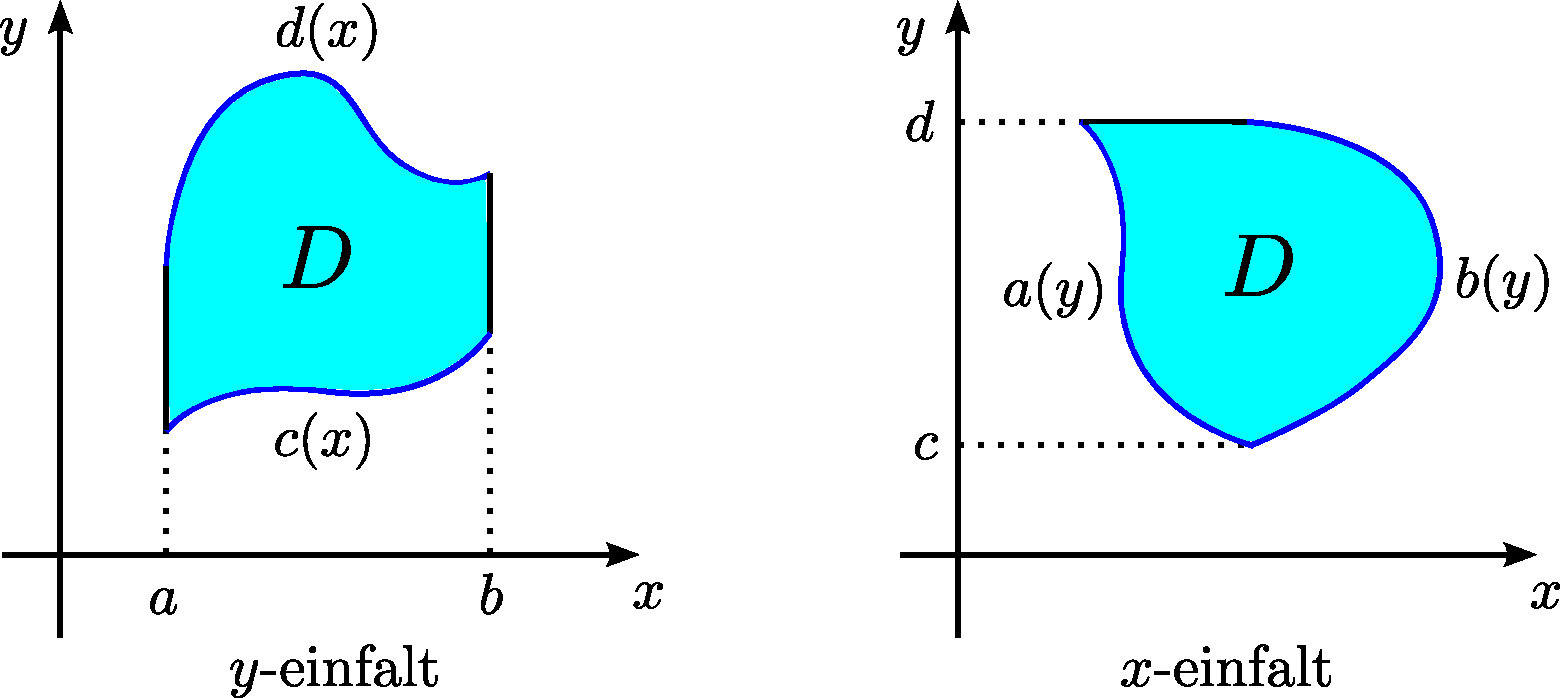
\includegraphics[width=0.65\linewidth]{einfalt}
            \caption*{}
\end {figure}



\subsubsection{Regla }
Lokað og takmarkað svæði $D$ í planinu er $y$-einfalt ef og aðeins ef sérhver lína af gerðinni $x=x_0$ sker $D$ í línustriki.  

\medskip
Lokað og takmarkað svæði $D$ er $x$-einfalt ef og aðeins ef sérhver lína af gerðinni $y=y_0$ sker svæðið í línustriki.



\subsection{Heildi yfir $x$-einföld og $y$-einföld svæði} 

\subsubsection{Setning }
Látum 
$D=\{(x,y)\mid a\leq x\leq b, c(x)\leq y\leq d(x)\}$
vera $y$-einfalt svæði og $f(x,y)$ fall sem er heildanlegt yfir $D$.  Þá er 
$$\tvint_D f(x,y)\,dA=\int_a^b\!\!\!\int_{c(x)}^{d(x)}f(x,y)\,dy\, dx.$$


\medskip
Látum 
$D=\{(x,y)\mid c\leq y\leq d, a(y)\leq x\leq b(y)\}$
vera $x$-einfalt svæði og $f(x,y)$ fall sem er heildanlegt yfir $D$.  Þá er 
$$\tvint_D f(x,y)\,dA=\int_c^d\!\!\!\int_{a(y)}^{b(y)}f(x,y)\,dx\, dy.$$



 \begin {figure}[h!]
 \centering
            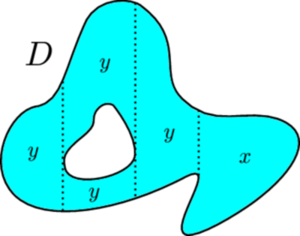
\includegraphics[width=0.35\linewidth]{einfalt2}
            \caption*{Hér er svæðinu $D$ skipt í endanlega mörg $x$-einföld og $y$-einföld svæði sem skarast eingöngu í punktum á jaðrinum.}
\end {figure}



\subsection{Óeiginleg heildi}
 \subsubsection{Umræða }
  Látum $f(x,y)\geq 0$ vera jákvætt fall sem er skilgreint á svæði $D$ í sléttunni. Ef
  \begin {enumerate}
   \item $D$ er ótakmarkað svæði eða
   \item $f(x,y)$ er ótakmarkað á $D$
  \end {enumerate}
má í sumum tilfellum skilgreina tvöfalda heildið af $f$ yfir $D$.

\medskip
Það er gert með því að finna fyrst runu af stækkandi lokuðum og takmörkuðum mengjum $D_1 \subseteq D_2 \subseteq \cdots \subseteq D$ sem 'stefnir á' $D$. Ef
\begin {equation*}
\tvint_{D_n} f(x,y)\,dA
\end {equation*}
er vel skilgreint fyrir öll $n$ og hefur markgildi þegar $n\to \infty$ (fyrir allar ólíkar runur $(D_n)_{n\geq 1}$) þá 
skilgreinum við \emph{óeiginlega heildið}
\begin {equation*}
 \tvint_{D} f(x,y)\,dA := \lim_{n\to \infty} \tvint_{D_n} f(x,y)\,dA .
\end {equation*}





\subsubsection{Skilgreining }
 Látum $f$ vera fall sem er heildanlegt yfir svæði $D$ í $\R^2$.  {\em Meðalgildi} fallsins $f$ á $D$ er skilgreint sem talan 
$$\bar{f}=\frac{1}{\mbox{flatarmál }D}\tvint_D f(x,y)\,dA.$$ 




\subsubsection{Skilgreining }
Svæði $D$ í $\R^2$ er sagt vera {\em
  samanhangandi} (e.~connected) ef um sérhverja tvo punkta $P_1$ og $P_2$ í $D$
gildir að til er ferill sem liggur í $D$, byrjar í $P_1$ og endar í
$P_2$.  (Hugtakið sem hér er skilgreint væri venjulega kallað {\em
  ferilsamanhangandi}.) 



\subsubsection{Skilgreining }
(Meðalgildissetning fyrir tvöföld heildi)
Gerum ráð fyrir að $f$ sé samfellt fall sem er skilgreint á lokuðu, takmörkuð og samanhangandi svæði $D$ í $\R^2$.   Þá er til punktur $(x_0,y_0)$ í $D$ þannig að 
$$\frac{1}{\mbox{flatarmál }D}\tvint_D f(x,y)\,dA=f(x_0,y_0).$$




\subsection{Breytuskipti} 

\subsubsection{Upprifjun }
 Látum $P=(x,y)\neq \ov$ vera punkt í plani.  {\em
  Pólhnit} $P$ er talnapar $[r,\theta]$ þannig að $r$ er fjarlægð $P$
frá 
$O=(0,0)$ og $\theta$ er hornið á milli striksins $\overline{OP}$ og
  $x$-ássins.  (Hornið er mælt þannig að rangsælis stefna telst
  jákvæð, og leggja má við $\theta$ heil margfeldi af $2\pi$.) 



\subsubsection{Skilgreining }
 {\em Pólhnitarétthyrningur} í $xy$-planinu
er svæði sem afmarkast af tveimur hringbogum $x^2+y^2=a^2$ og
$x^2+y^2=b^2$ og tveimur hálflínum sem byrja í $(0,0)$ og mynda hornin
$\alpha$ og $\beta$ við $x$-ásinn (Hornin eru mæld þannig að rangsælis
stefna telst jákvæð.) 
\begin {figure}[h!]
 \centering
            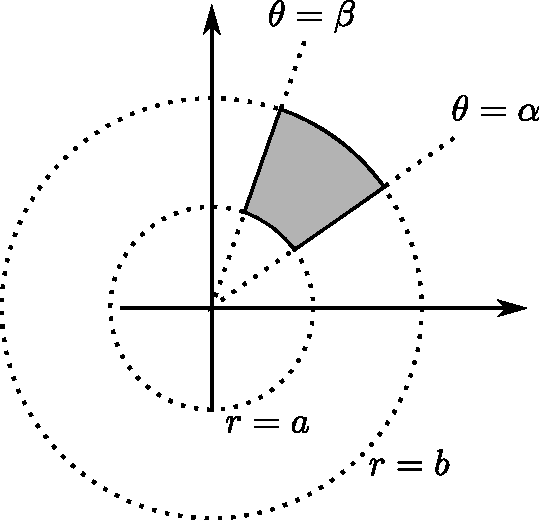
\includegraphics[width=0.35\linewidth]{polarrett}
	\caption*{}
\end {figure}
Gerum ráð fyrir að $0\leq a\leq b$ og að $0\leq\beta-\alpha\leq
2\pi$.  Þá má lýsa pólhnitarétthyrningnum með því  að nota pólhnit
þannig að 
$$D=\{[r,\theta]\mid 0\leq a\leq r\leq b, \alpha\leq \theta\leq\beta\}.$$
 



\subsubsection{Setning }
Ef $f$ er fall sem er heildanlegt yfir 
pólhnitarétthyrning
$D=\{[r,\theta]\mid 0\leq a\leq r\leq b, \alpha\leq \theta\leq\beta\}$
þá er 
$$\tvint_D f(x,y)\,dA=\int_\alpha^\beta\!\!\!\int_{a}^{b}
f(r\cos\theta,r\sin\theta)\,r\,dr\, d\theta.$$

\begin {figure}[h!]
 \centering
            \includegraphics[width=0.85\linewidth]{polarelement}
	\caption*{}
\end {figure}

\subsubsection{Upprifjun }
Látum $f$ vera fall skilgreint á bili 
$[\alpha,\beta]$.  Jafnan $r=f(\theta)$ lýsir mengi allra punkta í
planinu sem hafa pólhnit á forminu $[f(\theta),\theta]$ þar sem
$\alpha\leq\theta\leq\beta$.  Þetta mengi kallast {\em pólhnitagraf}
fallsins $f$. 


\subsubsection{Setning }
Látum $D$ vera svæði i $xy$-plani sem
afmarkast ef pólhnitalínum $\theta=\alpha$ og $\theta=\beta$ og
tveimur pólhnitagröfum $r=a(\theta)$ og $r=b(\theta)$.  Gerum ráð
fyrir að $0\leq a(\theta)\leq
r\leq b(\theta)$ og $0\leq \beta-\alpha\leq 2\pi$.
Ef $f$ er heildanlegt fall yfir $D$
þá er 
$$ \tvint\,f(x,y)\,dA=\int_\alpha^\beta\!\!\!\int_{a(\theta)}^{b(\theta)}
f(r\cos\theta,r\sin\theta)\,r\,dr\, d\theta.$$


\begin {figure}[h!]
 \centering
            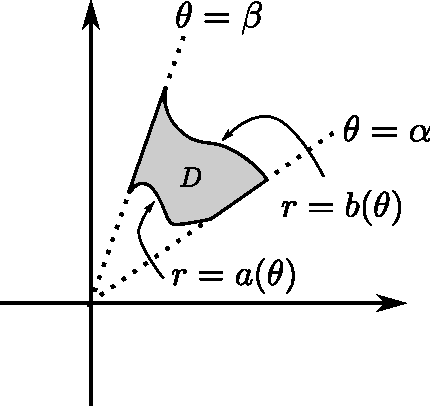
\includegraphics[width=0.35\linewidth]{polarsvaedi}
	\caption*{}
\end {figure}



\subsubsection{Regla }
Hugsum okkur að $f(x,y)$ sé fall og hægt sé að rita
$f(x,y)=g(x)h(y)$.  Látum $R=[a,b]\times [c,d]$.  Þá er 
\begin{align*}
\tvint_R f(x,y)\,dA&=\int_a^b\!\!\!\int_{c}^{d}g(x)h(y)\,dy\, dx\\
&=\bigg(\int_a^b g(x)\,dx\bigg)\bigg(\int_c^d h(y)\,dy\bigg).
\end{align*}

 

\subsubsection{Setning (Almenn breytuskiptaregla fyrir tvöföld heildi)}

Látum $x=x(u,v)$, $y=y(u,v)$ vera gagntæka vörpun milli svæðis $S$ í
$uv$-plani og svæðis $D$ í $xy$-plani.  Gerum ráð fyrir að föllin  
$x(u,v)$, $y(u,v)$ hafi samfelldar fyrsta stigs hlutafleiður á $S$.  Ef
$f$ er heildanlegt fall yfir $D$, þá er fallið $g(u,v)=f(x(u,v), y(u,v))$
heildanlegt yfir $S$ og 
$$\tvint_D f(x,y)\,dx\,dy=\tvint_S g(u,v)
\bigg|\frac{\partial(x,y)}{\partial(u,v)}\bigg|\,du\,dv.$$

\begin {figure}[h!]
 \centering
            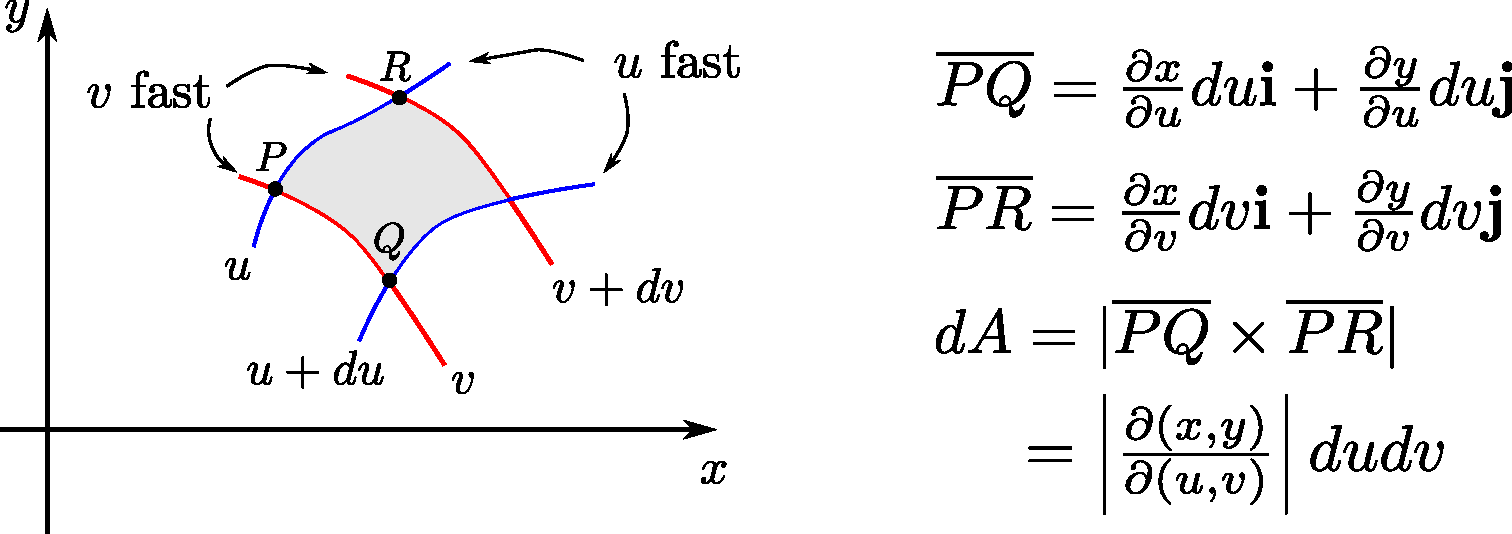
\includegraphics[width=0.85\linewidth]{changevar}
	\caption*{}
\end {figure}




\subsection{Þreföld heildi} 

\subsubsection{Umræða }
Heildi falls $f(x,y,z)$ yfir kassa $K=[a,b]\times[c,d]\times[u,v]$ í $\R^3$ er skilgreint á sambærilegan hátt og  tvöfalt heildi er skilgreint.  

\medskip
Á sama hátt og fyrir tvöföld heildi má svo skilgreina heildi fyrir almennari rúmskika í $\R^3$. 

\medskip
Heildi falls $f(x,y,z)$ yfir rúmskika $R$ er táknað með 
$$\thrint_R f(x,y,z)\,dV.$$
($dV$ stendur fyrir að heildað er með tilliti til rúmmáls.)



\subsubsection{Setning }
 Látum $f(x,y,z)$ vera fall sem er heildanlegt yfir kassa $K=[a,b]\times[c,d]\times[u,v]$ í $\R^3$.  Þá er
$$\thrint_K f(x,y,z)\,dV=
\int_a^b\!\int_c^d\!\int_u^v f(x,y,z)\,dz\,dy\,dx.$$ 
Breyta má röð heilda að vild, t.d.\ er 
$$\thrint_K f(x,y,z)\,dV=
\int_u^v\!\int_c^d\!\int_a^b f(x,y,z)\,dx\,dy\,dz.$$ 


\subsubsection{Setning }
 Látum $f(x,y,z)$ vera fall sem er heildanlegt yfir rúmskika $R$ og gerum ráð fyrir að $R$ hafi lýsingu á forminu
$$R=\{(x,y,z)\mid a\leq x\leq b,\ c(x)\leq y\leq d(x),\ u(x,y)\leq z\leq v(x,y)\}.$$
Þá er
$$\thrint_R f(x,y,z)\,dV=
\int_a^b\!\int_{c(x)}^{d(x)}\!\int_{u(x,y)}^{v(x,y)} f(x,y,z)\,dz\,dy\,dx.$$

Breyturnar $x, y, z$ geta svo skipt um hlutverk.



\subsubsection{Setning (Almenn breytuskiptaformúla fyrir þreföld heildi.) }
 Látum 
$$(u,v,w)\mapsto (x(u,v,w), y(u,v,w), z(u,v,w))$$
vera gagntæka vörpun milli rúmskika $R$ í $xyz$-rúmi og rúmskika $S$ í $uvw$-rúmi.  Gerum ráð fyrir að föllin $x(u,v,w), y(u,v,w), z(u,v,w)$ hafi öll samfelldar fyrsta stigs hlutafleiður.  Ef $f(x,y,z)$ er fall sem er heildanlegt yfir $R$ þá er
\begin {align*}
\thrint_R& f(x,y,z)\,dV \\&=\thrint_S f(x(u,v,w), y(u,v,w), z(u,v,w))
\bigg|\frac{\partial(x,y,z)}{\partial(u,v,w)}\bigg|\,du\,dv\,dw.
\end {align*}


\subsubsection{Skilgreining }
 Látum $(x,y,z)$ vera punkt í $\R^3$.  {\em Sívalningshnit} $(x,y,z)$ eru þrennd talna $r, \theta, z$ þannig að 
$$x=r\cos\theta\qquad\qquad y=r\sin\theta\qquad\qquad z=z.$$
Athugið að $[r,\theta]$ eru pólhnit punktsins $(x,y)$. 


\subsubsection{Setning (Breytuskipti yfir í sívalningshnit.)}

Látum $R$ vera rúmskika í $\R^3$ og látum $f(x,y,z)$ vera heildanlegt fall yfir $R$.  Gerum ráð fyrir að $R$ megi lýsa með eftirfarandi skorðum á sívalningshnit punktanna sem eru í $R$
$$\alpha\leq \theta\leq \beta,\ a(\theta)\leq r\leq  b(\theta), u(r,\theta)\leq z\leq v(r,\theta),$$ 
þar sem $0\leq \beta-\alpha\leq 2\pi$.  Þá er
$$\thrint_R f(x,y,z)\,dV= 
\int_\alpha^\beta
\!\int_{a(\theta)}^{b(\theta)}\int_{u(r,\theta)}^{v(r,\theta)}      
f(r\cos\theta,r\sin\theta,z)r\,dz\,dr\,d\theta.$$
 



\subsection{Kúluhnit} 

\subsubsection{Skilgreining }
 Látum $(x,y,z)$ vera punkt í $\R^3$.  {\em Kúluhnit} $(x,y,z)$ eru þrennd talna $\rho, \phi, \theta$ þannig að 
$$x=\rho\sin\phi\cos\theta\qquad\qquad y=\rho\sin\phi\sin\theta\qquad\qquad z=\rho\cos\phi.$$
Punktur sem hefur kúluhnit $\rho, \phi, \theta$ er táknaður 
með $[\rho, \phi, \theta]$. 

\begin {figure}[h!]
 \centering
            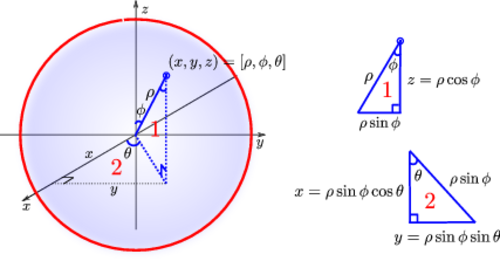
\includegraphics[width=0.75\linewidth]{sphere}
            \caption*{}
\end {figure}



\subsubsection{Umræða }
Eftirfarandi jöfnur gefa aðferð til að finna kúluhnit:
\begin{itemize}
\item[$\rho$]  er fjarlægðin frá $(0,0,0)$ til $(x,y,z)$, það er að segja 
$$\rho=\sqrt{x^2+y^2+z^2}.$$
\item[$\phi$] er hornið á milli jákvæða hluta $z$-ássins og línustriksins frá $(0,0,0)$ til $(x,y,z)$.  Hornið $\phi$ má ákvarða út frá jöfnunni
$$\tan\phi=\frac{\sqrt{x^2+y^2}}{z}.$$
\item[$\theta$] er hornið sem jákvæði hluti $x$-ásins myndar við línustrikið frá $(0,0,0)$ til $(x,y,0)$ (sama horn og notað í sívalningshnitum (og pólhnitum)).   Hornið $\theta$ má finna út frá jöfnunni
$$\tan\theta=\frac{y}{x}.$$
\end{itemize}
Um kúluhnit $[\rho, \phi, \theta]$ fyrir punkt $(x,y,z)$ gildir að 
velja má $\rho, \phi, \theta$ þannig að
$0\leq \rho$, $0\leq\phi\leq \pi$ og $0\leq\theta\leq 2\pi$.




\subsection{Breytuskipti í kúluhnit} 

\subsubsection{Setning }
 Látum $R$ vera rúmskika þannig að þegar notuð eru kúluhnit þá fæst eftirfarandi lýsing
$$R=\{[\rho,\phi,\theta]\mid \alpha\leq\theta\leq\beta, 
c\leq\phi\leq d, a\leq \rho\leq b\}.$$ 
Ef $f$ er fall sem er heildanlegt yfir $R$ þá er
\begin{align*}&\thrint_R f(x,y,z)\,dV=\\ &\int_\alpha^\beta\!\int_c^d\!\int_a^b f(\rho\sin\phi\cos\theta, \rho\sin\phi\sin\theta,\rho\cos\phi)
\,\rho^2\sin\phi\,d\rho\,d\phi\,d\theta.
\end{align*}




\subsection{Massamiðja} 

\subsubsection{Regla }
 Látum $D$ tákna svæði í plani.  Hugsum $D$ sem plötu þ.a.~í punkti $(x,y)$ er efnisþéttleikinn gefinn með falli $\delta(x,y)$.  Massi plötunnar er 
$$m=\tvint_D \delta(x,y)\,dA.$$
 {\em Vægi} plötunnar um línuna $x=0$ (þ.e.~$y$-ás) og um línuna $y=0$ (þ.e.~$x$-ás) eru gefin með
 $$M_{x=0}=\tvint_D x\delta(x,y)\,dA \quad \text{og} \quad M_{y=0}=\tvint_D y\delta(x,y)\,dA.$$

Hnit {\em massamiðju} plötunnar eru $(\overline{x}, \overline{y})$ þar sem 
$$\overline{x}=\frac{M_{x=0}}{m} \quad \text{og}\quad \overline{y}=\frac{M_{y=0}}{m}.$$




\subsubsection{Regla }
 Látum $R$ tákna rúmskika.  Hugsum $R$ sem hlut þannig að í punkti $(x,y,z)$ er efnisþéttleikinn gefinn með falli $\delta(x,y,z)$.  Massi hlutarins er 
$$m=\thrint_R \delta(x,y,z)\,dV.$$
 {\em Vægi} hlutarins um planið $x=0$ (þ.e.~$yz$-planið) er
 $$M_{x=0}=\thrint_R x\delta(x,y,z)\,dV.$$

Svipað skilgreinum við
 $$M_{y=0}=\thrint_R y\delta(x,y,z)\,dV \quad \text{og}\quad M_{z=0}=\thrint_R z\delta(x,y,z)\,dV.$$

Hnit {\em massamiðju} hlutarins eru $(\overline{x}, \overline{y}, \overline{z})$ þar sem 
$$\overline{x}=\frac{M_{x=0}}{m}
\qquad\mbox{og}\qquad
\overline{y}=\frac{M_{y=0}}{m}
\qquad\mbox{og}\qquad
\overline{z}=\frac{M_{z=0}}{m}.$$





\subsection{Hverfitregða} 

\subsubsection{Regla }
 Látum $R$ tákna rúmskika.  Hugsum $R$ sem hlut þannig að í punkti $(x,y,z)$ er efnisþéttleikinn gefinn með falli $\delta(x,y,z)$.  Látum $L$ tákna línu (snúningsás) í rúminu. {\em Hverfitregða} hlutarins um $L$ er
$$I=\thrint_R D^2 \,\delta\,dV$$
þar sem $\delta=\delta(x,y,z)$ og $D=D(x,y,z)$ er fjarlægð punktsins $(x,y,z)$ frá $L$.





\subsection{Yfirborðsflatarmál} 

\subsubsection{Regla }
 Látum $D$ vera svæði í plani og $f(x,y)$ diffranlegt fall skilgreint á $D$.  Flatarmál grafsins $z=f(x,y)$ þar sem $(x,y)\in D$ er gefið með formúlunni
$$S=\tvint_D \sqrt{1+f_1(x,y)^2+f_2(x,y)^2}\,dA.$$





\end{document}
